% description.tex
%-----------------
\clearpage
\section{Description}
\syn{SYNOPSIS}
\begin{verbatim}
	use Chart::type;     (type is one of: Bars, Composite,
	Direction, ErrorBars, HorizontalBars, Lines, LinesPoints,
	Mountain,	Pareto, Pie, Points, Split or StackedBars)
		
	$obj = Chart::type->new;
	$obj = Chart::type->new (width, height);
	
	$obj->set( $key_1, $val_1, ... , $key_n, $val_n);
	$obj->set( $key_1 => $val_1, ... , $key_n => $val_n);
	$obj->set( %hash );
	
	#GifGraph.pm-style API to produce png formatted charts
	@data = ( \@x_tick_labels, \@dataset_1, ... \@datase_n);
	$obj->png ( "filename", \@data );
	$obj->png ( $filehandle, \@data );
	$obj->png ( FILEHANDLE, \@data );
	$obj->cgi_png ();
	
	#Graph.pm-style API
	$obj->add_pt ($label, $val_1, ... $val_n);
	$obj->add_dataset ($val_1, ..., $val_n);
	$obj->png ("filename");
	$obj->png ($filehandle);
	$obj->png (FILEHANDLE);
	$obj->cgi_png();
	The similar functions are available for jpeg	
	
	#Retrieve imagemap information
	$obj->set('imagemap' => 'true' );
	$imagemap_ref = $obj->imagemap_dump();
	
\end{verbatim}
\clearpage
The Perl module \class{Chart} creates 'png' or 'jpeg' output which can be 
written into a file or output to 'stdout'. 
Therefore, \class{Chart} can also create dynamic charts for web sites.

It is possible to create a lot of different chart types, i.e., 
Bars, Composite, Direction, ErrorBars, HorizontalBars, Lines, LinesPoints, 
Mountain, Pareto, Pie, Points, Split and StackedBars.

Take a look at their descriptions to see how they work. 
All of the special types are classes by themselves. 
All these classes have the same abstract superclass: Base.pm. 
The hierarchy of Chart is shown in Figure~\ref{fig:Aufbau}.      

\begin{figure}[h]
	\begin{center}
		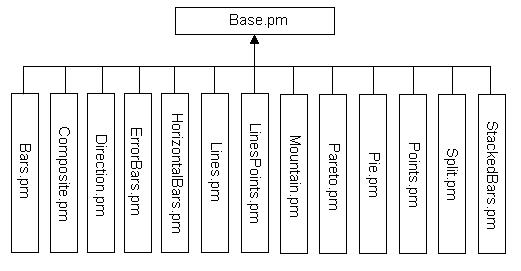
\includegraphics[scale=0.5]{Aufbau.png}
	\end{center}
	\caption{The hierarchy of chart}
	\label{fig:Aufbau}
\end{figure}

Therefore, you have to create an \emph{instance of one of the subclasses} 
to get a chart object.

All these methods and most of the options chart provides are implemented in Base. 
But the drawing of the graph itself happens in the respective subclass. 
Figure~\ref{fig:Elemente} shows the elements of a chart object.

\begin{figure}[h]
	\begin{center}
		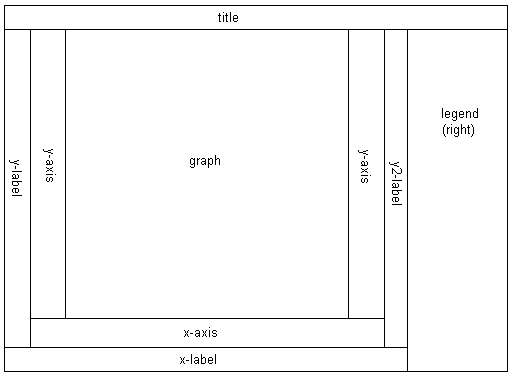
\includegraphics[scale=0.4]{Elemente.png}
	\end{center}
	\caption{Elements of a chart}
	\label{fig:Elemente}
\end{figure}

The graph area in the middle is drawn by the subclass, all the other elements are drawn by Base. 
But some classes don't need all of these elements or need special elements. 
Those elements have to be over-written in the respective class. 
For example, the class \class{Pie} doesn't need axes, 
so the methods for drawing the axes in file 'Base.pm' 
are over written by methods in class \class{Pie}; 
in this case no axes are drawn. 
Furthermore, the legend in a pie chart are a little bit different. Therefore Pie.pm has its
own methods for drawing the legends. These rules are managed by Chart. 
You don't have to attend to it. 

Chart uses Lincoln Stein's GD module for all its graphics primitives calls. 
So you need a installed version of GD.pm to use Chart. 
This module is like Chart available in the CPAN online archive at \kursiv{http://www.cpan.org/}.
\index{Lincoln Stein's GD module}    
